% ! TeX root = ...

\begin{frame}{Aggregate Computing}
  \begin{backgroundblock} 
    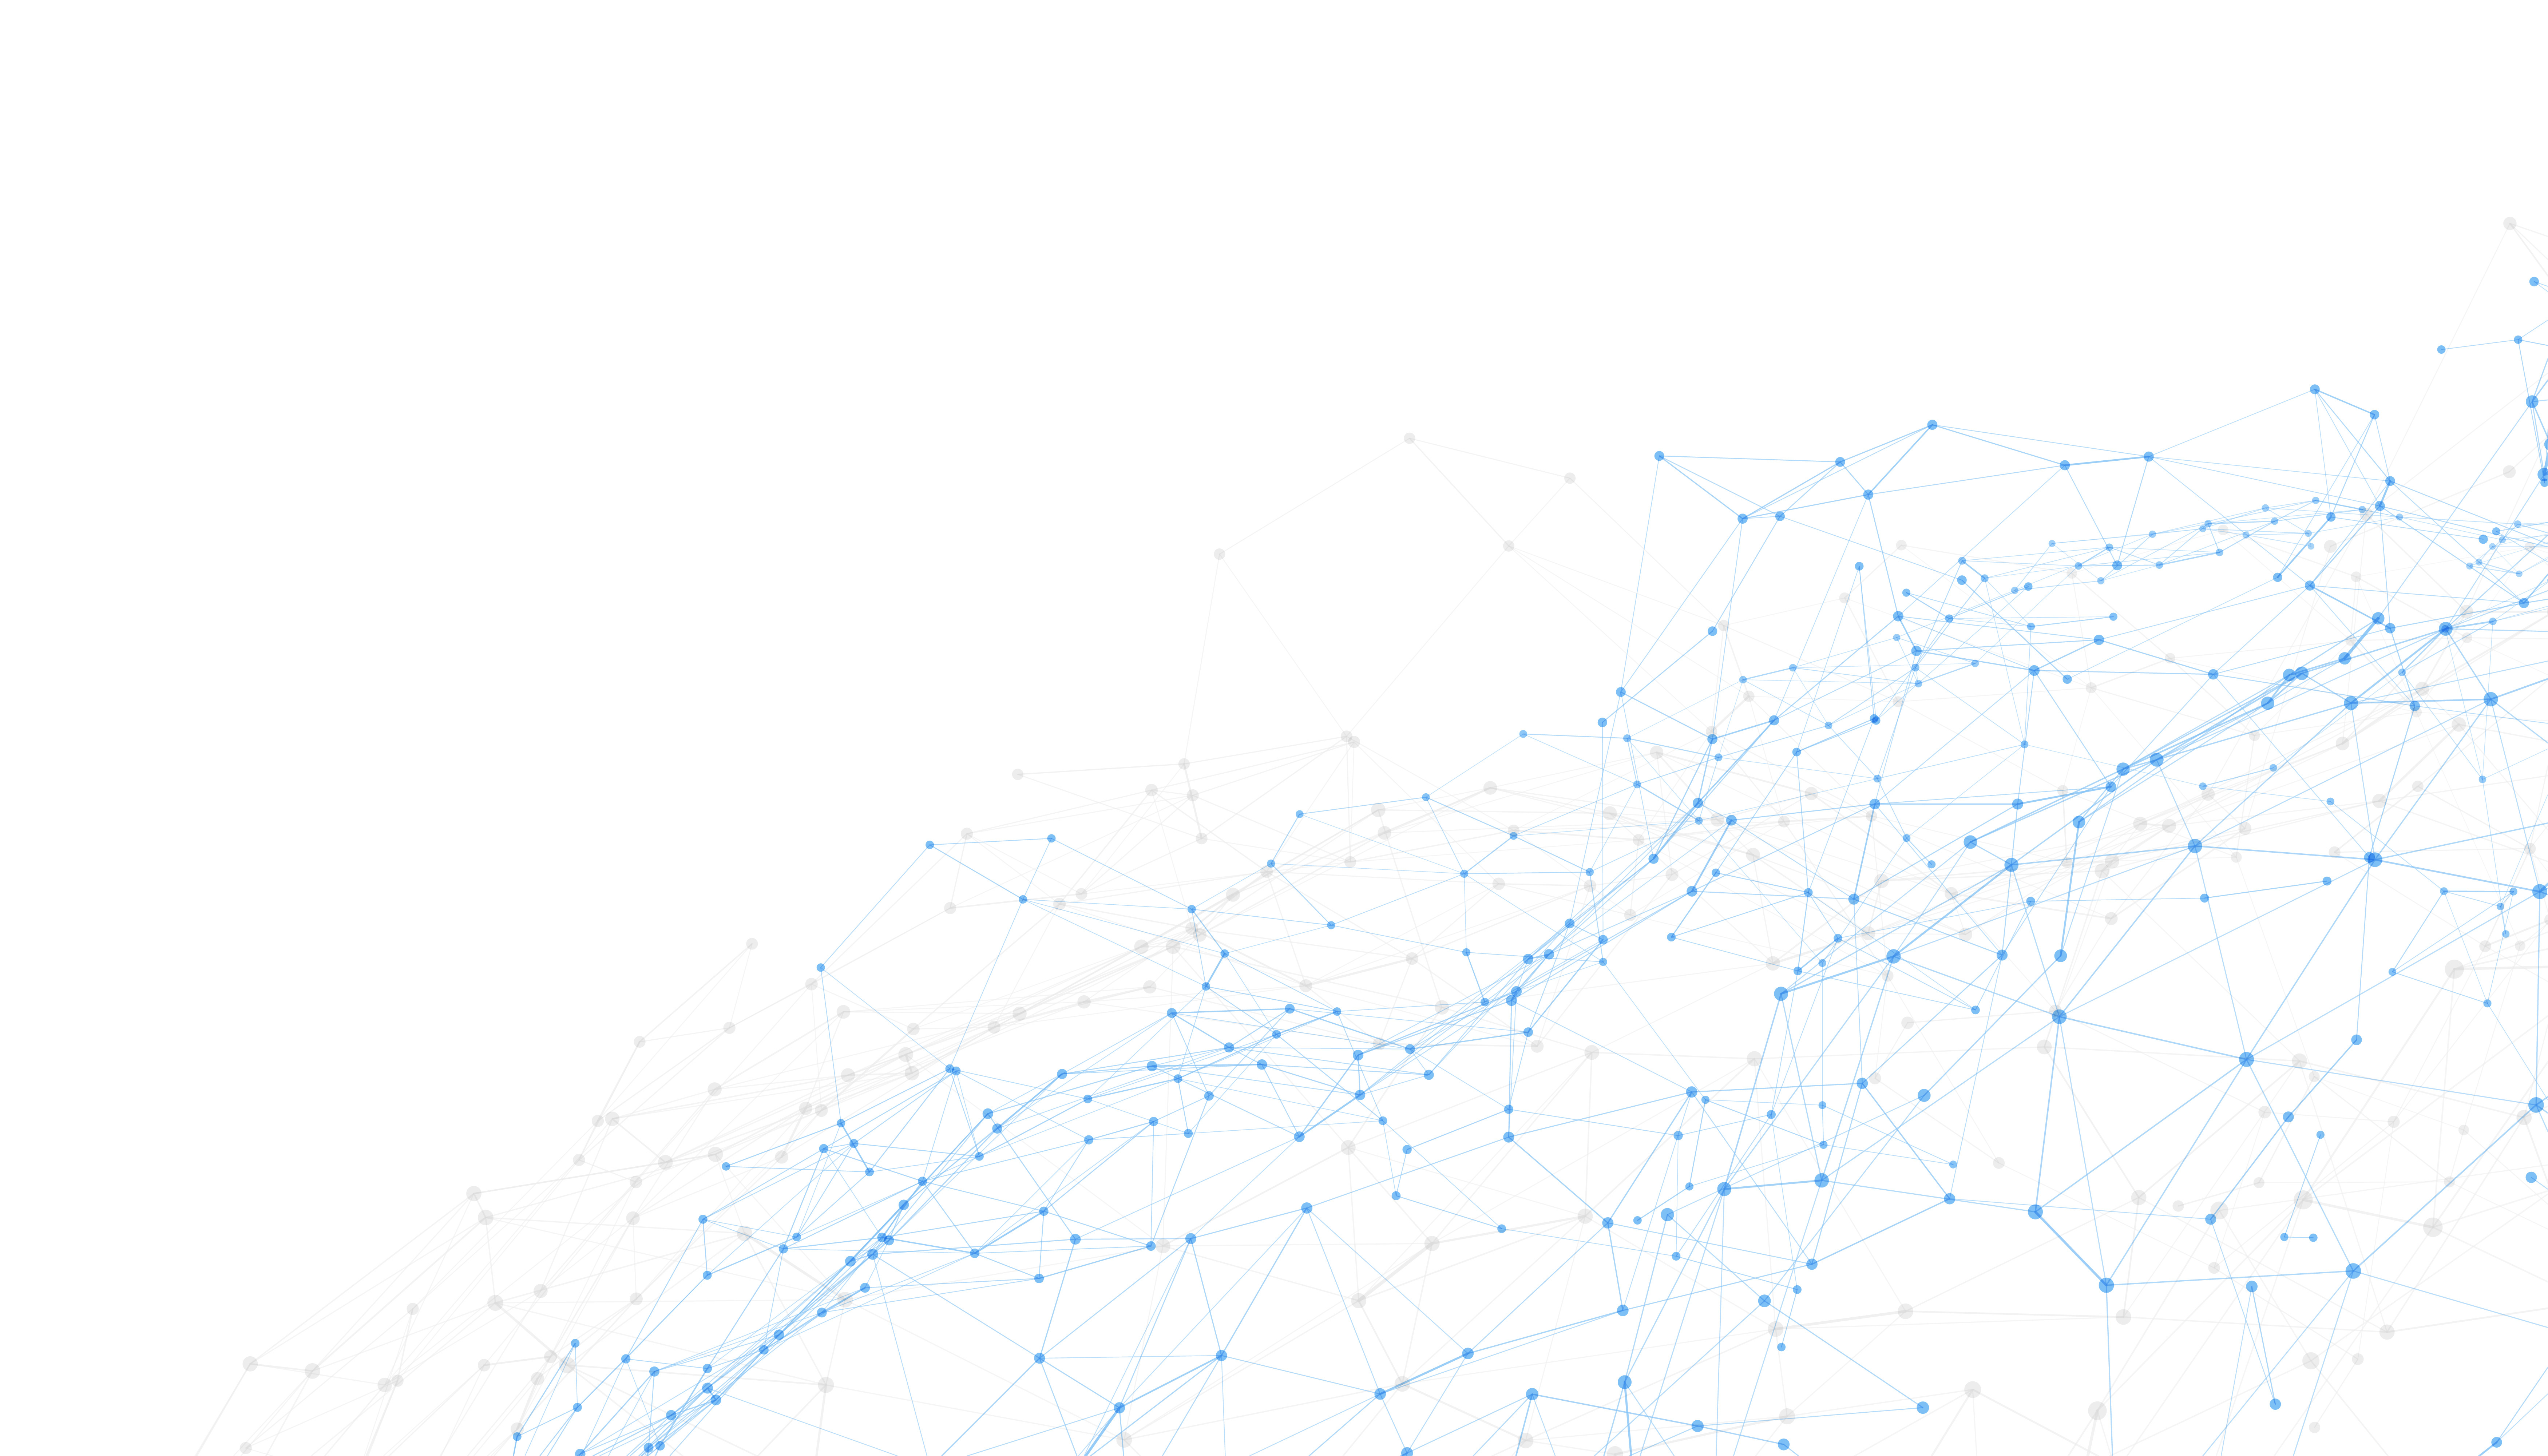
\includegraphics[width=\paperwidth]{img/aggregate-computing.jpg} 
  \end{backgroundblock} 
  \begin{card}
    \begin{itemize}
      \item <1-> A top-down global-to-local approach to express collective behaviour
      \item <2-> Rooted on \textit{field-calculus}
      \item <3-> Collective behaviour does not depends on system scale
      \item <4-> Used in various scenarios ranging from smart cities to crowd engineering
    \end{itemize}
  \end{card}
  \pause[5]
  \begin{cardRed}[\textbf{Problem} \faThumbsDown]
    \centering
    \textit{Building block design is hard}
  \end{cardRed}

  \pdfcomment{
    It is a top-down approach that makes it possible to coordinate large-scale, possibly heterogeneous, highly dynamic systems. 
    It mainly consists of manipulating a distributed data structure called Computational Field. 
    In contrast to swarm intelligent approaches, the idea here is to "program" the self-organisation by representing it as something like a first-class citizen of the language. 
    The program then can be split in each node, so that the collective behaviour can be easily scaled in very large systems (hundreds or thousands of nodes).
    A key advantage of this approach is its compositionality, which is inspired by functional programming.
    The paradigm is based on a small algebra called the field calculus, which expresses the minimal constructs that can be used to express any spatiotemporal computation.
    On top of this, we built intermediate-level abstractions, called Building-Block, which consist of the common patterns used in Aggregate Computing.
    We then used them to build domain-oriented applications to help developers express complex collective behaviour.
    Over the last ten/fifteen years, this methodology has grown rapidly. It is being used in many contexts such as crowd engineering, swarm robotics, and smart cities.
    Pragmatically, we see that it is not easy to develop building blocks that work well in different scenarios (e.g., high node mobility, uncertain environments).
    Sometimes it is a very tricky process of fine-tuning where we need to apply some constants to make our application work.
  }
\end{frame}